%% BioMed_Central_Tex_Template_v1.06
%%                                      %
%  bmc_article.tex            ver: 1.06 %
%                                       %

%%IMPORTANT: do not delete the first line of this template
%%It must be present to enable the BMC Submission system to 
%%recognise this template!!

%%%%%%%%%%%%%%%%%%%%%%%%%%%%%%%%%%%%%%%%%
%%                                     %%
%%  LaTeX template for BioMed Central  %%
%%     journal article submissions     %%
%%                                     %%
%%         <14 August 2007>            %%
%%                                     %%
%%                                     %% 
%% Uses:                               %%
%% cite.sty, url.sty, bmc_article.cls  %%
%% ifthen.sty. multicol.sty		   %%
%%				      	   %%
%%                                     %%
%%%%%%%%%%%%%%%%%%%%%%%%%%%%%%%%%%%%%%%%%


%%%%%%%%%%%%%%%%%%%%%%%%%%%%%%%%%%%%%%%%%%%%%%%%%%%%%%%%%%%%%%%%%%%%%
%%                                                                 %%	
%% For instructions on how to fill out this Tex template           %%
%% document please refer to Readme.pdf and the instructions for    %%
%% authors page on the biomed central website                      %%
%% http://www.biomedcentral.com/info/authors/                      %%
%%                                                                 %%
%% Please do not use \input{...} to include other tex files.       %%
%% Submit your LaTeX manuscript as one .tex document.              %%
%%                                                                 %%
%% All additional figures and files should be attached             %%
%% separately and not embedded in the \TeX\ document itself.       %%
%%                                                                 %%
%% BioMed Central currently use the MikTex distribution of         %%
%% TeX for Windows) of TeX and LaTeX.  This is available from      %%
%% http://www.miktex.org                                           %%
%%                                                                 %%
%%%%%%%%%%%%%%%%%%%%%%%%%%%%%%%%%%%%%%%%%%%%%%%%%%%%%%%%%%%%%%%%%%%%%


\NeedsTeXFormat{LaTeX2e}[1995/12/01]
\documentclass[10pt]{bmc_article}    



% Load packages
\usepackage{cite} % Make references as [1-4], not [1,2,3,4]
\usepackage{url}  % Formatting web addresses  
\usepackage{ifthen}  % Conditional 
\usepackage{multicol}   %Columns
\usepackage[utf8]{inputenc} %unicode support
%\usepackage[applemac]{inputenc} %applemac support if unicode package fails
%\usepackage[latin1]{inputenc} %UNIX support if unicode package fails
\urlstyle{rm}
\usepackage{nameref}
\usepackage{verbatim} 

\usepackage[table]{xcolor}
\usepackage{macros_tikz}


\definecolor{tableShade}{gray}{0.9}

 
 
%%%%%%%%%%%%%%%%%%%%%%%%%%%%%%%%%%%%%%%%%%%%%%%%%	
%%                                             %%
%%  If you wish to display your graphics for   %%
%%  your own use using includegraphic or       %%
%%  includegraphics, then comment out the      %%
%%  following two lines of code.               %%   
%%  NB: These line *must* be included when     %%
%%  submitting to BMC.                         %% 
%%  All figure files must be submitted as      %%
%%  separate graphics through the BMC          %%
%%  submission process, not included in the    %% 
%%  submitted article.                         %% 
%%                                             %%
%%%%%%%%%%%%%%%%%%%%%%%%%%%%%%%%%%%%%%%%%%%%%%%%%                     


%\def\includegraphic{}
%\def\includegraphics{}



\setlength{\topmargin}{0.0cm}
\setlength{\textheight}{21.5cm}
\setlength{\oddsidemargin}{0cm} 
\setlength{\textwidth}{16.5cm}
\setlength{\columnsep}{0.6cm}

\newboolean{publ}

%%%%%%%%%%%%%%%%%%%%%%%%%%%%%%%%%%%%%%%%%%%%%%%%%%
%%                                              %%
%% You may change the following style settings  %%
%% Should you wish to format your article       %%
%% in a publication style for printing out and  %%
%% sharing with colleagues, but ensure that     %%
%% before submitting to BMC that the style is   %%
%% returned to the Review style setting.        %%
%%                                              %%
%%%%%%%%%%%%%%%%%%%%%%%%%%%%%%%%%%%%%%%%%%%%%%%%%%
 

%Review style settings
%\newenvironment{bmcformat}{\begin{raggedright}\baselineskip20pt\sloppy\setboolean{publ}{false}}{\end{raggedright}\baselineskip20pt\sloppy}

%Publication style settings
%\newenvironment{bmcformat}{\fussy\setboolean{publ}{true}}{\fussy}

%New style setting
\newenvironment{bmcformat}{\baselineskip20pt\sloppy\setboolean{publ}{false}}{\baselineskip20pt\sloppy}

% Begin ...
\begin{document}
\begin{bmcformat}
 

%%%%%%%%%%%%%%%%%%%%%%%%%%%%%%%%%%%%%%%%%%%%%%
%%                                          %%
%% Enter the title of your article here     %%
%%                                          %%
%%%%%%%%%%%%%%%%%%%%%%%%%%%%%%%%%%%%%%%%%%%%%%

\title{Structure-based classification and ontology in chemistry}
 
%%%%%%%%%%%%%%%%%%%%%%%%%%%%%%%%%%%%%%%%%%%%%%
%%                                          %%
%% Enter the authors here                   %%
%%                                          %%
%% Ensure \and is entered between all but   %%
%% the last two authors. This will be       %%
%% replaced by a comma in the final article %%
%%                                          %%
%% Ensure there are no trailing spaces at   %% 
%% the ends of the lines                    %%     	
%%                                          %%
%%%%%%%%%%%%%%%%%%%%%%%%%%%%%%%%%%%%%%%%%%%%%%


\author{Janna Hastings\correspondingauthor$^1,^2$%
         \email{Janna Hastings\correspondingauthor - hastings@ebi.ac.uk}
       \and 
         Despoina Magka$^3$%
         \email{despoina.magka@cs.ox.ac.uk}%  logics
       \and
	     	 Colin Batchelor$^4$  % chemical ontology, text mining
	     	 \email{batchelorc@rsc.org}
       \and 
         Lian Duan$^1$%
         \email{dlian@ebi.ac.uk} %  chemoinformatics
       \and 
         Robert Stevens$^5$  % chemistry, ontology technology
         \email{robert.stevens@manchester.ac.uk}%
       \and 
         Marcus Ennis$^1$ % chebi
         \email{mennis@ebi.ac.uk}        
       and 
       	 Christoph Steinbeck$^1$%
         \email{steinbeck@ebi.ac.uk}%
      }
      

%%%%%%%%%%%%%%%%%%%%%%%%%%%%%%%%%%%%%%%%%%%%%%
%%                                          %%
%% Enter the authors' addresses here        %%
%%                                          %%
%%%%%%%%%%%%%%%%%%%%%%%%%%%%%%%%%%%%%%%%%%%%%%

\address{%
    \iid(1)Chemoinformatics and Metabolism, European Bioinformatics Institute, Hinxton, UK\\
    \iid(2)Swiss Center for Affective Sciences, University of Geneva, Switzerland\\
    \iid(3)Department of Computer Science, University of Oxford, UK\\
    \iid(4)Royal Society of Chemistry, Cambridge, UK\\
    \iid(5)Manchester University, UK%\\
}%

\maketitle

%%%%%%%%%%%%%%%%%%%%%%%%%%%%%%%%%%%%%%%%%%%%%%
%%                                          %%
%% The Abstract begins here                 %%
%%                                          %%  
%% Please refer to the Instructions for     %%
%% authors on http://www.biomedcentral.com  %%
%% and include the section headings         %%
%% accordingly for your article type.       %%   
%%                                          %%
%%%%%%%%%%%%%%%%%%%%%%%%%%%%%%%%%%%%%%%%%%%%%%


\begin{abstract}
        % Do not use inserted blank lines (ie \\) until main body of text.
\textbf{Background:} Recent years have seen an explosion in the availability of data in the chemistry domain. With this information explosion, however, retrieving \textit{relevant} results from the deluge of available information, and \textit{organising} those results, become even harder problems. Computational processing is essential to filter and organise the available resources so as to better facilitate the work of scientists. Ontologies encode expert domain knowledge in a hierarchically organised computable format. One such ontology for the chemical domain is ChEBI. ChEBI provides a classification based on structural features and a role or activity-based classification. An example of a structure-based class is `pentacyclic compound' (compounds containing five-ring structures), while an example of a role-based class is `analgesic', since many different chemicals can act as analgesics without sharing structural features. Structure-based classification in chemistry exploits elegant regularities and symmetries in the underlying chemical domain.  Some of these regularities lead easily to automated approaches to classification, and hierarchical organisation is available through clustering or scaffolding.  Logical definition of chemical classes in ontologies allows automated reasoning to detect class membership and manage hierarchies automatically.  Yet, some relevant and interesting chemical class types cannot yet adequately be automated by either the algorithmic or the logic-based methods.  As yet, there has been no systematic analysis of the types of structural classification in use in chemistry nor a comparison to the capabilities of available technologies.  

\textbf{Results:}  We analyze the different categories of structural classes in chemistry, presenting a list of patterns for features found in class definitions. These are xx, xx, xx, xx, xx and xx.  We compare these patterns of class definition to tools which allow for automation of hierarchy construction within chemoinformatics and within chemical ontology.  We find BLAH pattern is adequately treated in xx approach BLAH patterns in logic-based approach, and ... . Finally we discuss the relationships and interactions between chemoinformatics approaches and logic-based approaches. %Add some numeric quantifications

\textbf{Conclusion:} Systems which perform intelligent reasoning tasks need to rely on a diverse set of underlying computational utilities including algorithmic, statistical and logic-based tools.  For the task of automatic structure-based classification of chemical entities, essential to managing the vast swathes of chemical data being brought online, systems which are capable of hybrid reasoning combining several different approaches are crucial. We have provided a thorough review of the available tools amd methodologies, and identified several areas of open research questions, including. 


%%% OVERVIEW NOTE:
%The PROGRAM we are trying to define in this paper is the *types of definitions* (checklists), and the *arrangement of classes* defined using those types of definitions into a coherent, understandable hierarchy.  Within the program, arrange checks and marks.  Where marks, discuss ongoing research and DEFINE RESEARCH AGENDA. 

\end{abstract}



\ifthenelse{\boolean{publ}}{\begin{multicols}{2}}{}




%%%%%%%%%%%%%%%%%%%%%%%%%%%%%%%%%%%%%%%%%%%%%%
%%                                          %%
%% The Main Body begins here                %%
%%                                          %%
%% Please refer to the instructions for     %%
%% authors on:                              %%
%% http://www.biomedcentral.com/info/authors%%
%% and include the section headings         %%
%% accordingly for your article type.       %% 
%%                                          %%
%% See the Results and Discussion section   %%
%% for details on how to create sub-sections%%
%%                                          %%
%% use \cite{...} to cite references        %%
%%  \cite{koon} and                         %%
%%  \cite{oreg,khar,zvai,xjon,schn,pond}    %%
%%  \nocite{smith,marg,hunn,advi,koha,mouse}%%
%%                                          %%
%%%%%%%%%%%%%%%%%%%%%%%%%%%%%%%%%%%%%%%%%%%%%%




%%%%%%%%%%%%%%%%
%% Background %%
%%
\section*{Background}

Recent years have seen an explosion in the availability of data throughout the natural sciences. Primary data facilitates research through complex data-mining and knowledge discovery methods. However, with this information explosion, retrieving \textit{relevant} information from the deluge has become much more difficult. Computational processing is essential to filter, retrieve and organise such data. These goals are facilitated by \textit{formal ontologies}: machine-understandable encodings of human domain knowledge. These ontologies are used in several different ways \cite{lambrix2004}: to provide standardisation of terminology and identification across all entities in a domain so that multiple sources of data can be aggregated through comparable reference terms, to provide hierarchical organisation so that such aggregation can be performed at different levels and data can be browsed in an easily accessible fashion, and to allow for logic-based intelligent applications to be built which are able to perform complex reasoning tasks such as checking for errors and inconsistencies and deriving logical inferences. Logic-based knowledge representation (where ontologies serve as knowledge engineering artefacts) can be contrasted with algorithmic ``knowledge" representation, in which software algorithms procedurally define outputs based on stated inputs, and with statistical ``knowledge" representation, in which complex statistical models are trained to produce outputs based on a given set of inputs by learning weights for a complex set of internal parameters.  The advantages of logic-based knowledge representation is that it allows the knowledge to be expressed \textit{as knowledge}, i.e. as statements which are easily comprehensible, true and self-contained.  Statistical methods operate as black boxes and procedural methods require a programmer in order to manipulate or extend them. 

One example of a successful ontology in the biomedical domain is the Gene Ontology \cite{go2000}, which is used \textit{inter alia} for the statistical analysis of large-scale genetic data to identify genes which are significantly enriched for specific functions.  For the domain of biologically interesting chemistry, the Chemical Entities of Biological Interest ontology (ChEBI) \cite{chebi2010} provides a classification of chemical entities such as atoms, molecules and ions.  ChEBI organises chemical entities according to shared structural features, for example, carboxylic acids are all molecular entities that possess the characteristic carboxy group, and according to their activities in biological and chemical contexts, for example, acting as an antiviral agent. ChEBI is widely used as a database of chemical entities which can be queried both by structural classes and by functional annotations in the role ontology. The ontology has been applied in diverse applications such as annotation of chemicals in biological databases for pathways, interactions, and systems biology models \cite{matthews2009,libiomodels2010,kerrien2007}; chemical text mining \cite{corbett2006}; formalising the chemistry underlying biological ontologies \cite{mungall2010}; semantic similarity \cite{couto2010}; and metabolome prediction \cite{swainston2010}. Like the GO, ChEBI is manually maintained by a team of expert curators.  Historically, bio-ontologies such as GO and ChEBI have been developed as Directed Acyclic Graphs (DAGs), a deliberately simplified ontology format which allowed domain experts (non-logicians) to directly participate in ontology engineering at a time when tools with more sophisticated semantics were extremely difficult for non-technical persons to use. However, with the increasing availability of supporting tools and widespread adoption, there is a growing trend of evolution of bio-ontologies towards the Web standard ontology language OWL (Version 2) \cite{OWL2NextStep}, which provides a sophisticated suite of logic-based constructs to support eloquent knowledge representation and automated reasoning in real-world domains \cite{alterovitz2010}. 

Structure-based classification in chemistry exploits elegant regularities and symmetries in the underlying chemical domain.  Some of these regularities lead easily to algorithmic or statistical automated approaches to classification, and as a result, algorithmic approaches to hierarchical organisation of large-scale compound collections is a mature research area in chemoinformatics \cite{barnard1992,deshpande2005}. However, there are nevertheless several key benefits to adoption of the ontology-based approach in the chemistry domain, namely:
\begin{itemize}
	\item Classification knowledge represented in an ontology is \textit{explicit}, while algorithms which perform hierarchical classification often act as \textit{black boxes}, and to change the classification requires changes to the underlying software or re-training a complex statistical model.
	\item Using an ontology for classification allows for \textit{explanations} (justifications) \cite{horridgeentail09}, both for computed classifications and for computed inconsistencies. This can be contrasted to black-box approaches such as neural networks which cannot offer any explanations. 
	\item Representation of chemical knowledge in an ontology allows it to be harnessed in a generic fashion from within diverse knowledge-based applications which also utilize knowledge from \textit{other domains} (a core requirement for whole-scale systems biology), while to make use of chemoinformatics algorithms and toolkits requires custom software, differing from the software used in other domains.
	\item There are several types of chemical class definition which are not adequately represented in algorithmic approaches, but can be formalised in logical expressions (although not always in straightforward OWL). 
\end{itemize}

Conversely, there are several benefits to adopting chemoinformatics tools within the ontology engineering process in the domain of chemistry, such as to benefit from the well-developed and rapid algorithms for detecting parthood between chemicals and for computing properties.  In this paper, we present an analysis of the types of structure-based classes used in chemistry, and then discuss these as compared to available chemoinformatics algorithms for computing hierarchical ordering on sets of compounds and to the available constructions for encoding class definitions in chemical ontologies based on OWL.  We then explore aspects of chemoinformatics tools which we believe can enhance chemical ontology and explore problem areas in common to both fields which we believe can provide a stimulus for future research bridging the domains of chemoinformatics and computational logic. 


STATE PROBLEM AND MOTIVATION FOR THIS PAPER CLEARLY HERE:  A FULLY AUTOMATED CHEBI, A KNOWLEDGE-AWARE SYSTEM OF CLASS DEFINITIONS, SETTING OUT A RESEARCH AGENDA


The remainder of this paper is organised as follows. This Background presents some relevant chemistry and ontology preliminaries.  Following that, in our Results we firstly present the types of classes used in chemical classification and thereafter compare these types of classes to the capabilities of chemoinformatics hierarchy construction methods in chemoinformatics and that of chemical ontologies. In our Discussion, we further elucidate the relationship between chemoinformatics and logical approaches, and present some applications of chemical ontology.  We conclude with our outlook and open research areas. 



\subsection*{Classification in chemistry}
\label{sec:backclassif}

The ability to \textit{classify} raw information into meaningful groups is an essential component of human intelligence, which thus far has proven difficult to replicate in machine reasoning except in narrowly defined domains.  In particular, classification has a long tradition in chemistry:  the periodic table of the elements is one of the longest-standing and most-used systems of hierarchical classification throughout the natural sciences.  

%%% Colin says
The type of hierarchical classification that interests us here is classification of molecules into hierarchical groups based on which atoms in them are connected to which other atoms, or aspects of overall atomic constitution.  In both chemical synthesis in the lab and biosynthesis in organisms, the methods and pathways involved are entirely based on related structures, and this is why so many synthetic chemistry papers have titles which include some sort of systematically named description of a \textit{class} of chemicals, such as
\begin{itemize}
\item Synthesis of (pyrazolo)pyrimidines/pyridines
\item BOP-mediated one-pot synthesis of $C_5$-symmetric macrocyclic pyridone pentamers
\item Halonium-initiated electrophilic cascades of 1-alkenoylcyclopropane carboxamides: efficient access to dihydrofuropyridinones and 3(2$H$)-furanones
\item Spontaneous formation of a dibromoborenium cation driven by interaction between a borane Lewis acid and an arene $\pi$ system
\item Structural diversity for phosphine complexes of stibenium and stibinidenium cations
\end{itemize}

or a natural product based name such as a `polyketide' or a `spongistatin'.  This categorisation of chemical space is orthogonal to the sorts of classification more familiar in chemoinformatics analyses, which are largely machine-learning driven, and concentrate on whether a molecule is likely to bind to a particular site in a protein based on a heuristic analysis of large amounts of data. The latter types of classification are not relevant for the methods described in the current paper.  
%%%

The benefits of classification systems are severalfold. Classification \textit{organises} large volumes of information into sensible groupings so that they are more accessible to humans. Such hierarchical organisations can be more easily browsed; research in cognitive science shows that humans can only browse and compare a relatively low number of concepts at the same level at the same time, thus grouping into hierarchies reduces the amount of detail that has to be dealt with at each level \cite{sternberg2003}. A hierarchical structure allows narrowing in on the area of interest within a large domain, and only exploring the details of that narrowed in area, rather than observing the full domain at such a detailed level. A second benefit of a hierarchical organisation is that it allows for the compact representation of generalised knowledge at the highest level to which it applies.  For example, statements which are true for all mammals need to be expressed at the level of mammals as a whole, and not repeated for every specific mammal that occurs downstream.  Similarly, features which apply to all carboxylic acids can be expressed at the level of carboxylic acids as a whole, rather than repeated at the level of the different molecules as is required in databases or other flat structures which allow no general grouping or hierarchical organisation. 

Hierarchical organisation of knowledge in a domain allows for data-driven discovery, enabling useful predictions to be made.  For example, in functional genomics, the analysis of large-scale genetic data is facilitated by the grouping together of different genes which perform the same function, and modular analysis of such datasets reveals organisation at an aggregate level which is sometimes not apparent at the level of the raw data due to overloading of detail and noise in the underlying signal. %CITATION NEEDED
Hierarchical organisation of knowledge also allows useful predictions to be made, since it allows generalisation of knowledge to the highest possible level of applicability, and consequent prediction of properties of novel discovered members of the class.  

Chemical classes, the objects found within a chemical classification system, group together chemical entities in meaningful, scientifically relevant hierarchy. Ideally, all members of a chemical class should share important dispositional properties such as chemical reactivity. In fact, almost the only methods of classification available to historical chemists, before compound structures were well understood, were (i) based on the observation of reactivity through means of performing controlled reactions between different substances; or (ii) based on the origin of the molecule, when the molecule was isolated from a natural product substance. Much of these historical forms of classification are still inherited today and are taught in chemistry classes and reproduced in textbooks. Knowledge about the structural features which form the underlying causes of the shared dispositional properties (where such existed), and the structural features shared between similar natural product substances, was only developed later. However, now that chemical structures are well described (within the limits of the chemical graph formalism), many more structural features are able to be used for chemical class definitions. 

Interesting classes in chemistry can be grouped into those which are structure-based and those which are not. Structure-based classes are defined based on the presence of some shared structural feature across all members of the class.  This feature, however, may be crisply defined or vaguely defined.  Crisply defined structural classes will form the bulk of our focus in this paper, and are discussed further in the section \textit{\nameref{sec:resultsclasses}} below.   

Vaguely defined structural classes are those that are based on a family resemblance between a group of molecules, which are often of natural origin or have biological relevance.  For example, \textit{steroids} are defined as ``Any of naturally occurring compounds and synthetic analogues, based on the \textit{cyclopenta[a]phenanthrene carbon skeleton}, partially or completely hydrogenated; there are usually \textit{methyl groups} at C-10 and C-13, and often an \textit{alkyl group} at C-17. By extension, one or more bond scissions, ring expansions and/or ring contractions of the skeleton may have occurred."  The vagueness is indicated by terms and phrases such as `usually', `one or more' and `may have'.

Chemical classes can also be defined based on where the chemical came from in synthetic or natural pathways. Chemicals of natural metabolic origin are called \textit{natural products}.  As our ability to determine molecular structure by such methods as crystallography, NMR, CASE has improved over the past century, our ability to describe what is in a particular structural class has improved.  For example the Klymollins (doi:10.1021/np200589n), extracted from the coral \textit{Klyxum molle},
are all produced by reactions from a common core molecule and have very similar connectivities and compositions. This is a common pattern for recently-discovered natural product molecules.  Contrast this with alkaloids, one of the earliest classes of natural products to be identified, for which the best formal definition we have for the class reads ``Any of basic nitrogen compounds (mostly heterocyclic) occurring mostly in the plant kingdom (but not excluding those of animal origin). Amino acids, peptides, proteins, nucleotides, nucleic acids, amino sugars and antibiotics are not normally regarded as alkaloids. By extension, certain neutral compounds biogenetically related to basic alkaloids are included." A flexible and expressive language is needed to fully do justice to the wide range of class names which are intuitive to chemists and can be found in natural language such as in electronic lab notebooks such as are used in industry and indeed in more traditional scientific publications. 
%%%

Many interesting classes of chemicals are defined based on what the chemical does (its function or activity) in a biological or chemical context. Included in this group are drug usage classes such as antidepressant and antifungal; chemical reactivity classes such as solvent, acid and base; and biological activities such as hormone \cite{batchelor2010}. These are included in ChEBI under the `role' ontology. 

%Re: certain types of uncertainty in class definitions in terms of contextual information, perhaps can cite Bio-ontologies and OWLED papers, in the Discussion where the need for hybrid systems for knowledge representation are discussed. 

Hybrid classes are composed from an intersection of the members of two different classes, howsoever defined.  Examples are `tricyclic antidepressant', `tetracyclic antibiotic', 'organofluorine pesticide', 'pyrazole pesticide', 'organophosphorus pesticide' and 'thiourea pesticide'. Compositional entities such as these are easily dealt with by logical intersection, described further below. %(say something about OWL). %%INTRODUCE THIS IN THE LOGIC SECTION
Throughout this paper, we operate on the assumption of compositionality, which is a notion which goes back to Frege.  (Grundlage der Arithmetik, section 60: ``Es genuegt, wenn der Satz als Ganzes einen Sinn hat; dadurch erhalten auch seine Theile ihren Inhalt.'')
If there were compounds that were tricyclic and antidepressant but were not themselves `tricyclic antidepressant's, these would be violations of compositionality, because then there would be some extra condition not present in the name which would be necessary to decide whether something was itself a `tricyclic antidepressant'.
We know that compositionality works in chemistry because of the success of name-to-structure software such as Opsin \cite{lowe2011},
but for this to operate for hybrid classes for which some aspects of the class definition is not structural, then it needs a database of annotated chemicals to the non-structural classes, as is provided by ChEBI. 

% This is a background section. 
\subsection*{Logic-based reasoning and ontology}
\label{sec:backlogic}

Logic-based representation lies at the heart of modern knowledge representation (KR) technologies. It employs formal methods developed in the context of mathematical logic in order to encode knowledge about the world. The key requirement for these methods is that the knowledge is stored in a machine-processable format. Although a wide range of KR formalisms have been investigated, a core feature that KR languages share is the use of a well-defined syntax and semantics. The syntax serves as the alphabet of the language: it provides a set of symbols and a set of rules that regulate the arrangement of the symbols. The semantics enriches the syntactic objects with a meaning so that expressions satisfying a certain syntax have a universal and predefined interpretation. A set of such expressions, known as \textit{axioms}, that models domain-specific knowledge about an aspect of the world constitutes an \emph{ontology} in the computer-science sense. 

The amenability of KR languages to automated reasoning is of crucial importance. A reasoning algorithm -- relying on principles of logical deduction -- computes the inferences that follow from a set of formally defined axioms; note that a reasoning algorithm is tied uniquely to the specific syntax and semantics of a given KR language. A reasoning engine can be used to check the logical consistency of a set of logical axioms. For instance, if a knowledge base (i) defines organic and inorganic compounds as disjoint chemical classes (ii) contains the fact that cobalamin is an organic compound and (iii) also classifies cobalamin as inorganic, then a contradiction will be detected. Another standard reasoning task is the discovery of information that is not explicitly stated in the ontology. For example, if an ontology categorises cobalamin as B vitamin and also asserts that B vitamins participate in cell metabolism, then the fact that cobalamin participates in cell metabolism is derived. The automation of the above tasks -- traditionally performed by humans -- has a clear advantage as it permits the allocation of research resources to more intellectually satisfying activities.

A reasoning procedure needs to exhibit certain properties in order to be practically useful. Namely, a reasoning algorithm needs to derive \emph{correct} inferences, that is inferences which are in accordance with the semantics of the language; this property is known as \emph{soundness}. Additionally a reasoning algorithm ought to be \emph{complete}, i.e. to compute \emph{all} the correct inferences that are entailed by a set of axioms. Finally, an essential need for a reasoning algorithm is to \emph{terminate}, that is to halt after a finite amount of time. A vital contribution of logic is that it can offer guarantees -- by means of formal proofs -- for the soundness, completeness and termination of a reasoning algorithm for \emph{all} input ontologies. A KR formalism for which a sound, complete and terminating reasoning algorithm exists is (informally) called \emph{decidable}, though strictly speaking, according to the formal definitions of logic, it is the \emph{problem} of deciding whether a knowledge base is inconsistent that is (un)decidable, rather than the actual language. As a consequence, decidability is a highly desirable feature for a logic-based formalism to enable real-world applications.

Apart from decidability, another important feature of KR formalisms is tractability, that is how expensive the reasoning tasks are in terms of computational resources, e.g. performance time. The trade-off between the expressive power and the tractability of a logic-based language is a fundamental one: increasing the expressivity of the language usually results in a more resource-consuming reasoning algorithm or even undecidability. For instance, consider first-order logic (FOL) and propositional logic (PL): FOL allows one to model a much broader range of situations than PL, for example that for every molecule X, if X is organic and contains a hydroxyl group, then X is an alcohol, whereas in PL one may state an implication only for a \emph{specific} molecule. Nevertheless, reasoning in propositional logic is decidable, whereas reasoning tasks in unrestrained first-order logic are undecidable.

The need for decidable formalisms has been the driving force behind the development of Description Logics (DLs), a family of logic-based languages with well-understood computational properties that allow for different sorts of definitional statements when building a knowledge base. DLs serve as the underlying formalism for the Web Ontology Language (OWL) which is a W3C-standardised  knowledge representation language that is widely used both in industry and in academia; ontologies such as GO or ChEBI can be expressed in OWL. A powerful feature of OWL is the ability to perform \emph{automatic classification} based on \emph{full class definitions}. A full class definition is specified in terms of necessary and sufficient conditions for class membership. For instance, the OWL axiom \begin{equation}\mathsf{Molecule \sqcap MetallicCompound} \equiv \mathsf{Compound \sqcap \exists hasAtom.MetalAtom}\end{equation} states that an object is a metallic compound if and only if it is a compound and it has a metal atom. Due to the machine-understandable nature of OWL definitions, OWL is the standard knowledge representation and reasoning language for use in the Semantic Web, which differentiates itself from the Syntactic Web by associating Web documents with a well-defined meaning. Significant advances in the DL research led to the release of OWL 2\footnote{http://www.w3.org/TR/owl2-overview/} which improves on the first version of OWL by providing new expressive features, such as more advanced handling of data values and ranges (such as qualified cardinality restrictions and property chains).
%The readership has no idea what qcrs and pcs are.  Make use of later, or scrub.

A DL ontology may include two kinds of logic-based axioms: expressions that encode conceptual knowledge about the world (also known as \emph{TBox axioms}) and instance level statements that describe a particular situation (also known as \emph{ABox axioms}). An example of a TBox axiom is \begin{equation} \mathsf{ \exists hasPart.Carboxyl} \sqsubseteq \mathsf{CarboxylicAcid}\end{equation} which says that if a molecule has a carboxyl part, then it is a carboxylic acid. On the other hand, the set $\mathsf{hasPart(m,p),Molecule(m),Amine(p)}$ gives ABox axioms that describe \emph{one} particular molecule which is explicitly named in the ontology (the molecule $\mathsf{m}$).

In spite of the fact that OWL is a very efficient KR formalism for the encoding of tree-like structures (i.e. those whose `branches' do not rejoin), it is fundamentally unable to correctly represent cyclic structures, such as molecular entities containing ring structures \cite{magka2010}.
% This is a deeper result to do with the Chomsky hierarchy---necessarily OWL axiomata are expressed in a context-free language and cycles are necessarily context-sensitive.  Surely someone has noticed this before that paper?  At least I noticed it *years* ago but never provided a proof; sorry.
OWL exhibits the tree-model property \cite{VardiModalLogic} which on the one hand ensures important computational properties, such as decidability, but on the other hand prevents the users from describing non-tree-like %non-context-free - sort this out! Ask Nooshi.
structures using OWL axioms. For instance, one may state using OWL axioms that cyclobutane has four carbon atoms, but it is not possible to specify that these four atoms are arranged in a ring. Therefore, one of the prevailing challenges in chemical knowledge representation is crafting logic-based formalisms that are able to faithfully represent cyclic structures and, thus, pave the way for ontology-based applications that automatically classify chemical compounds.


\section*{Results}

\subsection*{Types of features used to structurally define chemical classes}
\label{sec:resultsclasses}

The chemical graph formalism \cite{trinajstic1992} allows the description, in so far as the molecule is well-described using valence bond theory, of fully defined chemical classes at a certain level of granularity, for example, the class of all paracetamol molecules.  Paracetamol molecules all have in common the connectivity as described in the graph describing the class, but individual molecules vary in conformation and configuration depending on their environmental context. The chemical graph formalism, however, only applies to fully defined chemical structures, and there are limited extensions to support higher-level modelling (such as R groups). 

%There are many different types of classes that are used in chemistry, for various reasons of historical development and usefulness. New classes are both created and discovered; just as research in natural chemistry and biochemistry reveals new information, so too synthetic chemists are able to create ever more complex and creative structures.

By examination of the definitions of higher-level structural classes included in ChEBI, we have identified the following categories of elementary features used in structural chemical class definitions: 
\begin{enumerate}
	\item	Interesting parts (IP), such as the carboxy group or the cholestane scaffold
	\item	Basic chemical properties (CP), such as the charge of the entire species
	\item	Which atoms are present (AP)
	\item	Topological features (TF), such as rings, chains and fused ring systems
	\item Mechanical connectivity and shape (MC), such as rotaxanes, host--guest compounds, catenanes and cage compounds
	\item	Schemata for structural formulae (SF) such as C$_n$H$_{2n}$.
\end{enumerate}

Most of these elements can be used singly or in combination with other elements via compositionality.  Further explanations as well as examples follow in the sections below. For clarity, the classes and examples are summarised in \textit{\nameref{tab:classes}}, where each feature is assigned a unique code that will be used in the sections that follow.

\subsubsection*{Interesting parts (IP)}

%Chemists probably think in terms of skeleta, substituents and spacers.  Spacers are important in materials chemistry and connect different bits of skeleton together.  [add examples]

Perhaps the most prominent of methods for classifying chemical entities based on features of their structures is based on the presence or absence of specific parts.  Such parts may be the overall `skeleton' of the structure or they may be minor constituents. The skeleton is usually loosely defined as the major or most relevant part of the molecule, the `backbone' to which other groups are attached as decorations. 

For example, `metalloporphyrin' is defined as any compound containing a porphyrin skeleton and a metal atom.  Note that as the term is commonly used in chemistry, a skeleton is not always a straightforward substructure, since bonds may be added or removed while retaining more or less the same skeleton, with perhaps different degrees of saturation. Allowing for different degrees of saturation, or the addition or removal of parts of the skeleton, gives rise to a vague class definition. Here, therefore, we focus on the stronger sense of skeleton that implies that the skeleton as specified must be a substructure of the molecule it is a skeleton of. Classes defined with skeleta in this fashion are often named for the skeleton, such as `porphyrin' for the compound and the class `porphyrins'. Indeed, the same name is often used to mean a single compound, a class of compounds with the skeleton of that compound, and the larger class of compounds containing a part which has that skeleton \cite{corbett2008}. 

Parts may also be straightforward constituents in which there is no implicature that the part is somehow maximal, as there is in the case of skeletons.  General parts are termed `groups' (which may be simple atoms). The number (count, cardinality) of such groups is also important.  For example, tricarboxylic acids can be defined as a compound containing exactly three and no more than three carboxy groups.  With regard to the cardinality of groups within a molecule, a challenge that is absolutely key to machine-based classification in chemistry, less so in biology with the exception of those things that are basically chemical (such as RNA) is \textit{scalar implicature}. Scalar implicature means that when one specifies a number, that number is the maximal description of the number of entities of interest. For example, while it is literally true that I have one leg, normal behaviour is to say that I have two legs. The chemical parallels run something like this: if you are working in material science or developing liquid crystals, or are interested in lipids in biological systems, you will make extensive use of alkyl chains which are chains of methylene (CH2) groups.  It is trivially true that a chain of $n$ methylene groups is also a chain of ($n-1$) methylene groups.  However, it would be misleading to describe a molecule with a dodecyl group attached as a methylated compound simply because it contains a substructure with the formula CH$_3$ at the end of the alkyl chain. 

%%% Colin says
%Grice (1975) discusses speech acts, in terms of a principle of cooperativity, which is to say that human speakers tend to be cooperative when they communicate in the sense of minimising the amount of work that needs to be done by the listener. Grice further elaborates this in terms of a set of four maxims, and the maxim that interests us here is the maxim of relation, which is roughly that ones communication should be as informative as possible but without being more informative than is needed.  [Grice's maximum of quantity here]
%%%

The class definition may also specify the position at which a group (or set of groups) is attached to a skeleton. Such positions are assigned by rules for numbering the skeleton of a molecule in a reproducible (and community-agreed-upon) fashion.  %For example, \ldots 
% see iupac pages at qmul.ac.uk (g p moss) for examples of numbering systems

Some particularly problematic classes refer to the relative arrangement of parts / attachments within the whole molecule. A special case is the relative configuration of stereocentres. Chemical graphs can be specified for completely stereochemically specified entities, and for completely stereochemically unspecified entities, but relative configurations of stereogenic centers cannot be specified using traditional chemical graph representation formalisms. For example, `allothreonine' [\textit{rel}-(2$R$,3$R$)-2-amino-3-hydroxybutanoic acid] and `threonine' [\textit{rel}-(2$R$,3$S$)-2-amino-3-hydroxybutanoic acid] are compounds with a relative configuration of stereogenic centres, thus for which a graph cannot currently be drawn. What cannot be represented in the graph formalism is a relative arrangement of these - if one is up, the other is down - or if one is down, the other is down - for example. 
\textit{gem}-diols are those diols, compounds with exactly two hydroxy groups, where both hydroxy groups are attached to the same atom.  Similarly, $\alpha,\beta$-unsaturated alcohols have a double bond between the bond bearing the hydroxy group (the $\alpha$ atom) and one of its immediate neighbours (the $\beta$) atom. $\alpha,\omega$-disubstituted compounds have substituents of interest to the chemist at either end of the molecule, regardless of its length.

\subsubsection*{Basic chemical properties such as charge (CP)}

Straightforward chemical properties such as charge and number of unpaired electrons are used to define broad classes of molecules such as ion and radical. The latter are particularly of interest to chemists working in the gas-phase, particularly in atmospheric chemistry, where hydroxy radicals play an important role in mopping up air pollution and can even be smelt at certain times of day. Aromaticity and saturation are other properties commonly found in class definitions. These also apply at a lower level of classification, such as `aromatic diazonium ion'.  

Wihle aromaticity as a property is commonly algorithmically determined based on alternating patterns of single and double bonds within ring structures, we should note that there are edge cases for which aromaticity may not necessarily be safely inferred given a particular substructure. This is particularly true for large or heavily substituted systems (see Rzepa \textit{passim}).


\subsubsection*{Which atoms are present (AP)}

Classes may be defined based on the presence of certain types of atoms, organised according to the layout of the periodic table.  Examples are `carbon molecular entities' and `lanthanoid molecular entities'. Classes qualify as subclasses of carbon molecular entities if they contain any atom of carbon, regardless of what other atoms they contain in addition.  Classes qualify as subclasses of lanthanoid molecular entities if they contain any of the lanthanoid group atoms.  As most complex molecular entities belong to several such classes, automation of this aspect of classification is obviously highly desirable. 


\subsubsection*{Topological features (TF)}

Another element commonly used in class definitions is the number and arrangement of rings (cycles) in a ring system which is a part of the molecule. For example, the classes `ring assembly' and `polycyclic cage' both refer, in their definitions, to numbers and arrangements of rings in the molecule. Polycyclic cages are molecules which are composed entirely of cycles which are fused together in such a way as to form an overall cage-like structure.  Examples are the fullerenes, cucurbiturils -- so named for their similarity to pumpkins, nanotubes, and small regular compounds such as cubane.  Polycyclic compounds are also named for the number and counts of rings they contain, e.g. tetracyclic or  pentacyclic. The manner in which the 

\textit{ortho}- and \textit{peri}-fused compound: A polycyclic compound in which one ring contains two, and only two, atoms in common with each of two or more rings of a contiguous series of rings. Such compounds have $n$ common faces and fewer than $2n$ common atoms.  \textit{ortho}-fused compound: A polycyclic compound in which two rings have two, and only two, adjacent atoms in common. Such compounds have $n$ common faces and $2n$ common atoms.

Related to the chemical properties from the previous section, the `cyclic' modifier is often treated as an overall property of the molecule and as a modifier for other class types. Consider: `cyclic ketone', `cyclic peptide', %homo- versus hetero- here, possibly
 `cyclic ether', `cyclic tetrapyrrole', \ldots

\subsubsection*{Mechanical connectivity and shape (MC)}

Chemicals defined based on shapes: Molecular M\"{o}bius strips and knots such as catenanes, rotaxanes and trefoil knots.

Look at Fraser Stoddart's stuff. 


\subsubsection*{Structural formulae (SF)}
\label{sec:molformula}

Another form of definition by atomic composition is the definition of classes of molecular entity based on specifying the \textit{exclusive} atomic composition.  This can be contrasted to parthood (where other attachments are allowed). 

Finally, an interesting, yet problematic to depict with existing graph-based tools, element of chemical class definitions, is that based on structural formula. 

For example, `alkane' is defined as ``an acyclic branched or unbranched hydrocarbon having the general formula C$_{n}$H$_{2n+2}$.'' 

Also, macromolecules (strings of repeating units). % there are two sorts of definition; see the Purple Book; source-based and structure-based. 

%\subsubsection*{Hybrid classes}

%Given all of the above different types of elements of chemical class definitions, perhaps the most interesting classes arise in combinations of the various different elements, including combinations of structure-based class elements and non-structure-based groupings:  tricyclic antidepressant; tetracyclic antibiotic and so on...





% IS THERE A PROBLEM WITH NON-COMPOSITIONALITY HERE?
%%
%%  Compare the above class types to the various available methods of automatic hierarchy construction in chemoinformatics
%%  Intended to also serve as a related work review on classification methods in chemoinformatics
%%
\subsection*{Algorithmic and statistical approaches to automatic hierarchy construction}
\label{sec:resultscheminf}

%The interesting question, which is not yet addressed in the below -- given the above types of chemical class definitions, and their implied hierarchical relationships, to what extent can the existing chemoinformatics approaches construct hierarchies in which the nodes correspond to classes defined in the above way? 

Chemoinformatics solutions have been developed to classify sets of chemical entities automatically.
What do they do?  A key area is quantitative structure--activity relationships (QSAR). These seek to find robust relationships between substructures, both of the graph-theoretic sort described above, and pharmacophores, which are arrangements of interesting atoms in three-dimensional space, and a given biological activity.

Such automatic classification systems are in common use in industry, particularly drug discovery, agrochemicals and <UNILEVER/>.  Algorithms for automated classification tend not work well on arbitrary graph-based data structures, so they reduce graphs to characteristic \textit{features} or \textit{descriptors}, which serve as the input for classifiers. 

As defined by Todeschini and Consonni\cite{Todeschini2000}, a molecular descriptor is the final result of a logical and mathematical procedure which transforms chemical information encoded within a symbolic representation of a molecule into a useful number (calculated descriptors), or, the result of standardized experiments (experimental descriptors). Among the calculated descriptors, if we focus on structural features, molecular fingerprints are binary strings in which each bit represents a feature.  In the most common types of fingerprint, a feature could be either a pre-defined substructure or a random substructure mapped by a hashing algorithm.

In hierarchy construction algorithms, such as \textit{hierarchical similarity clustering} \cite{Adamson1991,barnard1992}, feature sets are clustered on the basis of high mutual pairwise similarity along a particular dimension.  Either agglomerative methods, where all instances are assigned their own class and these classes merged, or divisive methods, where everything is assigned to a single class and this class subdivided, can be used.

The results depend both on the feature-identification algorithms and on the similarity calculations between resulting feature sets. There are many different algorithms for computing similarity measures between compounds and for aggregating compounds into clusters based on pairwise similarity measures, leading to arbitrarily many different classification hierarchies, even given the same compound collection as input.  A limitation of such an analysis is that each node in the hierarchy represents a class with an arbitrary meaning, lacking a formal definition.  The tree is highly sensitive to changes in input structures and the calculated features, making it very difficult to compare results across datasets even when the same clustering and fingerprinting algorithms are used. Another limitation is that most feature sets on which similarity measures are calculated, in order to be efficiently computable, represent only a subset of the total features of the molecules concerned, and local paths through the structures predominate over the (more expensive) overall molecular structure. Thus, molecules may turn out to appear quite similar according to such an algorithm (due, perhaps, to a predominance of similar parts) while displaying rather different structures overall.  This problem is exacerbated for molecules of high structural regularity (e.g. polycyclic carbon compounds).  Nevertheless, similarity landscapes are of paramount importance %WHY? - explain why for drugs - also remember that drug discovery is awfully voodoo and the lab chemists will optimize the fuck out of a given lead and give you something entirely different
in reducing the complexity and understanding the features of large collections of compounds when using such an approach.
 
%To what extent are / should SMARTS and R-GROUPS be relevant here?
% Sit down with the SMARTS spec and show what it can do with definitions
% But note that it doesn't give you hierarchies because IT IS NOT COMPOSITIONAL.  So C cannot be derived from X.
% Markush notation was invented to baffle and bullshit the enemy.

All the above is basically rule-based but machine learning approaches to QSAR have become fashionable recently. Supervised methods, such as Bayesian classifiers, decision trees and support vector machines, are employed to classify compounds for a particular functional activity class.  However, these approaches, resulting as they do in binary output, do not immediately lend themselves to hierarchical classifications.  Supervised machine learning for prediction of chemical class membership based on an existing hierarchy is an interesting option but have hitherto only been shown to work (HELLO?) on small numbers of classes, and furthermore requires a reasonably large training set of chemicals which are already classified.  Although existing databases like ChEBI and MeSH~\cite{meshUrl} could act as training sets for such an endeavor, the size of these data is still a tiny fraction of the enormous chemical space, and the problem is further complicated by the fact that the leaf nodes of such classification trees normally contain few structures. Also the ChEBI classification, at least, is far from complete. An arbitrary compounds belongs to loads, literally loads of classes and will only have been classified under one or two. 

%Machine learning has to be further discussed.  In particular the way that machine learning allows application of certain types of hierarchy construction on a larger scale than exhaustive pairwise alignment?  

% SCAFFOLDS (PARTHOOD)
Beyond feature-based, similarity-based and statistical approaches to automatic classification, an additional approach in common use in chemoinformatics is classification based on substructures~\cite{deshpande2005}.  A substructure represents a wholly contained part of a molecule, and characteristic molecular substructures (skeletons or scaffolds and attached groups) are usually highly correlated with characteristic activities.  Nodes in hierarchies based on substructures are able to be labelled with the relevant substructure that is shared for all members of the class, thus, have more meaning to humans than statistical or similarity-based classes. Variants on this approach include Maximum Common Substructure (MCS) based clustering and scaffold tree clustering. LibraryMCS~\cite{librarymcs} is a commercial application that can perform MCS based clustering on a set of structures. Although the technical details of the underlying implementation are not available, from the output it can be determined that structures sharing a common substructure are organized in the same class, and the common substructures define the scope of each class.  Scaffold Tree~\cite{Schuffenhauer2007} is a product which hierarchically classifies scaffolds, which are molecular frameworks obtained by removing side chains.  By recursive removal of rings in scaffolds, scaffolds are decomposed into smaller ones which form the higher levels in the hierarchy tree.  

Both MCS- and scaffold-based methods are very helpful in visualizing and giving an overview of a given dataset.  Furthermore, the intermediate nodes which represent shared scaffolds or MCS structures correspond to the definition of classes based on an important part.  These definitions could be extracted and formalized.  But the output of these algorithmic approaches is still highly dependent on the input, thus could not act as a universal chemical classification system. (Even if it were possible to guarantee that the input corresponded to the universal chemical space, it is likely that the consequence would be a non-terminating classification algorithm.)  These approaches are generally directly useful, since scaffolds often specify the general overall structure of the molecule, which in bioactive and especially in synthetic chemistry has a large influence on the activity of the molecule in the biological system.  However, hierarchies based on scaffolding do not allow for the specification of overall properties of the molecule, nor for clustering based on similar aspects of molecules aside from their scaffolds.  

Scaffolds resemble skeletons, and MCS- and scaffold-based approaches come close to automatic construction of hierarchies for classes defined based on interesting parts of the molecule.  Can check those boxes in the classification wishlist. 

% CRB: TODO: look at book from Sheffield cheminformatics course and add appropriate citations. Schuffenhauer stuff maybe too recent for same.

% Further limitations?



% The concept of scaffold may be as vague as skeleton;  it may be that X-containing entities are classified or instead that entities that are largely or mostly X are classified. If the latter, it would be very interesting to see how this is defined, as this can help us.  If the former, it is very similar to the approach which Leo and Michel have developed and reported on (to be cited later).





%%
%%  Compare the above class types to the various available methods of classification in chemical ontologies
%%  Intended to also serve as a related work review on chemical ontology
%%
\subsection*{Automatic classification in chemical ontologies}
\label{sec:resultschemontology}

%% DESPOINA TO HELP WITH THIS SECTION
We discussed previously how automated reasoning techniques can be used to define chemical classes in the context of an ontology and to construct an appropriate hierarchy. 
In the current section we take a closer look and we investigate a number of KR formalisms--and in some cases implemented applications--that have been used for the purpose of classification of molecules based on their structure.  For each logic, we pinpoint the limitations of its expressive power by inspecting a number of examples. 
We therefore analyse the advantages and the drawbacks of each suggested formalism and estimate its usefulness in practice.

% Assuming a background in which full class definitions expressed in chemical ontologies enables automated reasoning both to check class membership and to construct appropriate hierarchies, to what extent do the logical facilities available to ontologies allow the construction of definitions according to the patterns outlined above? 
% 


\subsubsection*{Interesting parts}


The representation and classification of chemical molecules based on the presence of specific functional groups is among the most well-developed areas of ontology-based chemical applications. One of the first uses of OWL technology for chemical classification purposes is reported by Dumontier et al \cite{dumontier2007}, where chemical molecules, described by means of the atoms and bonds that they contain, are grouped into ontological classes that are defined by virtue of functional groups. Note that the functional groups of a molecule determine its chemical reactivity and are identified by the existence of certain substructures in the molecular graph. In the aforementioned work, a hierarchy of chemical classes was built through the structural specification of certain functional groups; subsequently, ontological assertions were extracted (with the help of a software tool) from molecular descriptions that are given in a standard chemoinformatics representation formalism. Finally, molecules are classified under chemical classes with the help of the extracted assertions and an OWL reasoning engine. The main expressive feature of OWL that this approach takes advantage of is the full existential quantification, that is the ability to define chemical classes based on the existence of parts of some sort; for instance, a compound is a carboxylic acid if and only if there \emph{exists} a part in this compound \emph{that is of the kind} carboxyl.

However, due to the inherent inability of OWL to faithfully describe non-tree-like patterns, it was not possible to encode  the inner structure of functional groups with rings, such as benzene rings. Dumontier et al. suggest a workaround of this deficiency using DL-safe rules \cite{dumontier2007}; nonetheless, as we discuss in detail in Section~\ref{subsubsec:cycles} ``Cycles and ring arrangements'', circumscribing OWL's inability to represent cycles with DL-safe rules offers an only partially satisfactory solution. Finally, the FOL-style semantics of OWL prevent the modeller from defining chemical classes based on the absence of specific parts. A typical example of this category are hydrocarbons, that is organic compounds that consist \emph{entirely} of hydrogen and carbon. As we illustrate in Section~\ref{subsubsec:entire} ``Properties based on entire molecular structures'' , it is necessary to leave the confines of OWL and of open-world semantics in order to specify the relevant classes. 

Overall, while not capturing many essential features of chemical classes and far smaller than ChEBI ontology, the discussed ontology\footnote{The URI of the OWL ontology \cite{dumontier2007} is \url{http://ontology.dumontierlab.com/cfg}.} achieves to classify arbitrary molecules in a defined hierarchy and, thus, presents a novel and promising methodology on the manipulation of chemical knowledge. In the same spirit, the Lipid Ontology, which encodes classes of lipids using OWL axioms, is geared towards automatic classification of lipids \cite{chepelevlipids2011}.
 


 

% The representation of, and classification of, chemicals based on their interesting parts in the form of functional groups is probably the most well developed area of OWL-based chemical ontology at present. Dumontier et al. \cite{dumontier2007} developed an ontology of chemical functional groups encoded in OWL, which was able to be used to automatically link chemical entities defined by means of graphs to ontological classes defined by means of functional groups. They made use of a cheminformatics software application to extract functional groups from molecules with chemical structures specified in standard cheminformatics representation formalisms. While not as rich as the feature term representation described above, and far smaller than ChEBI ontology, the Dumontier representation allows powerful use to be made of the relatively compact knowledge base of functional groups in terms of the classification of arbitrary molecules in a defined hierarchy. Care, however, had to be taken to only encode the structures of the functional groups insofar as they were not cyclic. Along similar lines is the OWL encoding used by the Lipid Ontology \cite{chepelevlipids2011} for automatic classification of lipids. 


\subsubsection*{Atomic composition}

Robert Stevens describes an OWL-ification of the periodic table here: http://robertdavidstevens.wordpress.com/2011/05/05/an-ontology-of-the-periodic-table-using-electronic-structure-of-the-atom/

\subsubsection*{Basic chemical properties}

A number of chemical classes are specified using numerical features of chemical entities, such as charge or mass. OWL 2\footnote{\url{http://www.w3.org/TR/owl2-syntax/#Datatype_Maps}} offers facilities for advanced handling of data values--widely known as datatypes--, such as integers or strings. Datatypes allow knowledge engineers to define classes by referring to particular (ranges of) values: for example, one may define \emph{small} molecules as the molecules whose molecular weight is less than 800 Daltons. Furthermore, OWL 2 reasoners provide datatype reasoning support\cite{Motik2008} in order to exploit this knowledge and derive new inferences: if it is stated that the weight of atropine is 289 Daltons, then atropine is automatically classified as a small molecule. Therefore, numerical information about molecules can be naturally integrated in an OWL 2 knowledge base and thus to eliminate the need for external chemoinformatics tools that may cause interoperability problems. This is a convenient feature in applications such as e.g. drug discovery, that require filtering out molecules below a critical weight. For instance, one may want to retrieve all the small tetrapyrroles molecules, that is compounds that contain four pyrrole rings and with weight less than a threshold value; ontology-based platforms enable researchers to perform such queries in a seamless and uncomplicated way.

\subsubsection*{Cycles and ring arrangements}
\label{subsubsec:cycles}

One of the first attempts to overcome the limitations of OWL to represent cycles was the DL-safe rules \cite{DLSafeBoris}. The extension of OWL ontologies with DL-safe rules arose as a formalism that allowed to perform certain reasoning tasks over non-tree-like structures while preserving decidability. Nevertheless, the restrictions that are necessary in order to enforce decidability restrain the applicability of the rules to only explicitly named objects of the ontology--that is individuals that appear in the ABox axioms. We illustrate this by means of an example: assume a simplified knowledge base whose contents appear in Table~\ref{tab:DL-safe-example}.\footnote{In the rest of the paper, we assume that there is an extra axiom stating that the roles $\mathsf{SingleBond}$ and $\mathsf{DoubleBond}$ are symmetric.} 
%

%MOVED to end ... as per template requirement

\begin{comment}

\begin{table}[t]
\centering
\caption{DL-safe rules example}\label{tab:DL-safe-example}
\rowcolors{1}{tableShade}{white}
\begin{tabular}{|l|l|}
    \hline
    TBox axiom    & $\mathsf{\exists hasAtom.RingAtom \sqsubseteq CyclicMolecule}$ \\
    ABox axioms & $\mathsf{Benzene(m),singleBond(a_1,a_2),doubleBond(a_2,a_3),singleBond(a_3,a_4),doubleBond(a_4,a_5),}$ \\ 
     & $\mathsf{singleBond(a_5,a_6),doubleBond(a_6,a_1),Carbon(a_i),hasAtom(m,a_i)}$  for each $ 1 \leq \mathsf{i} \leq 6$ \\
     DL-safe rule &  $\mathsf{ \bigwedge_{1 \leq i \leq 6}   Carbon(x_i)   \wedge singleBond(x_1,x_2) \wedge doubleBond(x_2,x_3) \wedge singleBond(x_3,x_4)} \wedge{}$ \\
     & $\mathsf{doubleBond(x_4,x_5) \wedge singleBond(x_5,x_6) \wedge doubleBond(x_6,x_1) \rightarrow RingAtom(x_1)}$ \\
      
     \hline 
\end{tabular}
\end{table}
%

\end{comment}

An inference engine will derive the assertion $\mathsf{CyclicMolecule(m)}$ but not the subsumption $\mathsf{Benzene \sqsubseteq CyclicMolecule}$. This example shows how the DL-safe rules extension does not allow to deduce subclass relations that concern \emph{all} the benzene molecules, that is to reason about the \emph{schema} of the ontology. 

In order to address the need for schema-level reasoning over structured objects as outlined above, a further OWL extension was suggested that combines OWL, rules and \emph{Description Graphs} (DGs), a new modelling primitive for the representation of complex structures  \cite{mghs09graphs-journal}. Let us present how DGs augment the expressive power of OWL with the help of an example. Assume that one models the benzene ring with the following OWL axiom, which states that an object is a benzene ring if and only if it has exactly six carbon atoms each of which has a single bond with exactly one carbon atom and a double bond with exactly one carbon atom. 
$$ \mathsf{BenzeneRing \equiv (= 6) hasAtom. (Carbon \sqcap (= 1) hasSingleBondWith.Carbon \sqcap (= 1) hasDoubleBondWith.Carbon)}$$
Figure~\ref{fig:benzene}(a) shows the ``canonical'' model of the benzene ring according to the OWL semantics: informally, the canonical model is a conceptual representation of what the logical definition of benzene ring encodes with as little information derivable from the logical formula as possible. The shape of the canonical model plays an important role, as it determines the subclass relations that are entailed by the knowledge base: the more accurately the canonical model represents a molecular structure, the richer the outputed hierarchy for this molecule is. If one chooses to describe the benzene ring with the help of DGs, the respective canonical model is the one that appears in Figure~\ref{fig:benzene}(b) which, in contrast to the model of Figure~\ref{fig:benzene}(a), manages to capture the underlying cyclic structure. This has significant benefits as additional inferences can be drawn and additional chemical classes that depend on ring structures can be defined within the DG formalism. As a direct consequence of the increased expressivity, a number of syntactic restrictions are enforced to the axioms of the knowledge base in order to guarantee decidability. One of these restrictions is the \emph{strong separation requirement} that prevents the user from mixing properties used in the OWL ontology with properties used in the DGs axioms. Therefore, if one uses the property $\mathsf{hasSingleBondWith}$ in the DGs formulas, then 
$\mathsf{hasSingleBondWith}$ may not occur in e.g. an axiom of the form $\mathsf{hasSingleBondWith} \sqsubseteq \mathsf{hasBondWith}$. The DGs formalism has been implemented and the implementation has served as the basis for a java tool that performs structure-based classification over the chemical entities of the ChEBI ontology. Although, this is one of the few OWL-based applications where cyclic structures are described with adequate precision, the range of chemical classes that can be axiomatised is somewhat limited by the constraints imposed by the underpinning formalism, such as the strong separation requirement.

%% Converted to straight image, sadly, as per BMC journal requirements.  The figure itself will need to be excluded from the PDF in the final version for submission -- and included in the submission as a separate file.  But I leave it in for now (at the end of the document)


\begin{comment}

\begin{figure}[t] 
\centering  
\begin{tabular}{l}
%%%%%%%%%%OWL MODEL%%%%%%%%%%%%%%%%%%%%%%%%%%%%%%%%%%%
\begin{tikzpicture}[thick]
\node
(cb)at(6.25,5.25)[thinLineEmptyRec,label=right:$\hspace{5mm} \mathsf{BenzeneRing}$]{};

\node (c1a) at (0,4)[thinLineEmptyRec,label=above:$\mathsf{Carbon}$] {};
\node (c1b) at (-0.5,3.25) [thinLineEmptyRec,label=below:$\mathsf{Carbon}$] {};
\node (c1c) at (0.5,3.25)[thinLineEmptyRec,label=below:$\hspace{10mm}\mathsf{Carbon}$] {};

\node (c2a) at (2.5,3)[thinLineEmptyRec,label=above:$\mathsf{Carbon}\hspace{10mm}$] {}; 
\node (c2b) at(2.,2.25) [thinLineEmptyRec,label=below:$\mathsf{Carbon}\hspace{5mm}$]{};
\node (c2c) at (3,2.25)[thinLineEmptyRec,label=below:$\hspace{5mm}\mathsf{Carbon}$] {};

\node (c3a) at (5,4)[thinLineEmptyRec,label=right:$\mathsf{}$] {}; 
\node (c3b) at(4.5,3.25) [thinLineEmptyRec,label=below:$\mathsf{Carbon}\hspace{5mm}$] {}; 
\node (c3c) at (5.5,3.25)[thinLineEmptyRec,label=below:$\hspace{1mm}\mathsf{Carbon}$] {};
\node (c3clabel) at (6,4.25) []{$\mathsf{Carbon}$};

\node (c4a) at (7.5,4)[thinLineEmptyRec,label=left:$\mathsf{}$] {}; 
\node (c4b) at (7.,3.25)[thinLineEmptyRec,label=below:$\mathsf{Carbon}$] {};
\node (c4c) at (8.,3.25) [thinLineEmptyRec,label=below:$\hspace{5mm}\mathsf{Carbon}$] {};
\node (c4clabel) at (6.5,3.75) []{$\mathsf{Carbon}$};

\node (c5a) at (10,3)[thinLineEmptyRec,label=above:$\mathsf{Carbon}$] {}; 
\node (c5b) at(9.5,2.25) [thinLineEmptyRec,label=below:$\mathsf{Carbon}\hspace{5mm}$]{};
\node (c5c) at (10.5,2.25)[thinLineEmptyRec,label=below:$\hspace{5mm}\mathsf{Carbon}$] {};

\node (c6a) at (12.5,4)[thinLineEmptyRec,label=above:$\mathsf{Carbon}$] {}; 
\node (c6b) at (12.,3.25)[thinLineEmptyRec,label=below:$\mathsf{Carbon}\hspace{10mm}$] {};
\node (c6c) at (13.,3.25) [thinLineEmptyRec,label=below:$\mathsf{Carbon}$] {};

 
\draw [->,densely dashed] (cb) -- (c1a);
\draw [->,densely dashed] (cb) -- (c2a);
\draw [->,densely dashed] (cb) -- (c3a);
\draw [->,densely dashed] (cb) -- (c4a);
\draw [->,densely dashed] (cb) -- (c5a);
\draw [->,densely dashed] (cb) -- (c6a);

\draw [-] (c1a) -- (c1b);
\draw [-,double] (c1a) -- (c1c);

\draw [-] (c2a) -- (c2b);
\draw [-,double] (c2a) -- (c2c);

\draw [-] (c3a) -- (c3b);
\draw [-,double] (c3a) -- (c3c);

\draw [-] (c4a) -- (c4b);
\draw [-,double] (c4a) -- (c4c);

\draw [-] (c5a) -- (c5b);
\draw [-,double] (c5a) -- (c5c);

\draw [-] (c6a) -- (c6b);
\draw [-,double] (c6a) -- (c6c);

\node (caption) at (6,0.25) [] {(a) Canonical model with the OWL definition};
\end{tikzpicture}
\\


\begin{tabular}{ll}
%%%%%%%%%%%DGs MODEL%%%%%%%%%%%%%%%%%%%%%%%%%%%%%%%%%%%
\begin{tikzpicture}[thick]
\node (cb) at (0.84,1.25)[thinLineEmptyRec,label=above:$\mathsf{BenzeneRing}$]{};
\node (c1) at (0.84,0.48) [thinLineEmptyRec,label=below:$\mathsf{Carbon~}$] {};
\node (c2) at (1.68,0) [thinLineEmptyRec,label=right:$\mathsf{~Carbon}$] {};
\node (c3) at (1.68,-1) [thinLineEmptyRec,label=right:$\mathsf{Carbon}$] {} ;
\node (c4) at (0.84,-1.48) [thinLineEmptyRec,label=below:$\mathsf{Carbon}$] {};
\node (c5) at (0,-1) [thinLineEmptyRec,label=left:$\mathsf{Carbon}$] {};
\node (c6) at (0,0) [thinLineEmptyRec,label=left:$\mathsf{Carbon~}$] {};

\draw [-,double] (c1) -- (c2);
\draw [-] (c2) -- (c3);
\draw [-,double] (c3) -- (c4);
\draw [-] (c4) -- (c5);
\draw [-,double] (c5) -- (c6);
\draw [-] (c6) -- (c1);

\draw [->,densely dashed] (cb) -- (c1);
 \draw [->,densely dashed] (cb) -- (c2);
 \draw [->,densely dashed] (cb) to [bend left=60]  (c3);
\draw [->,densely dashed] (cb) to [bend right=30] (c4);
\draw [->,densely dashed] (cb) to [bend right=60] (c5);
\draw [->,densely dashed] (cb) to (c6);
\node (caption) at (-1,-2.75) [] {(b) Canonical model with the DGs definition};
\end{tikzpicture}
&
%%%%%%%%%%%CHEMICAL GRAPH%%%%%%%%%%%%%%%%%%%%%%%%%%%%%%%%%%% 
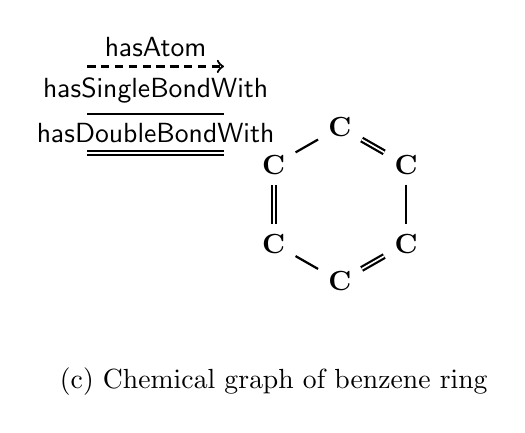
\begin{tikzpicture}[thick]
\node (e1) at (-2.5,2.25) [] {};
\node (e2) at (-0.5,2.25) [] {};
\draw [->,densely dashed] (e1) -- (e2) node[midway,above]{$\mathsf{hasAtom}$};
\node (e1) at (-2.5,1.65) [] {};
\node (e2) at (-0.5,1.65) [] {};
\draw [-] (e1) -- (e2) node[midway,above]{$\mathsf{hasSingleBondWith}$};
\node (e1) at (-2.5,1.15) [] {};
\node (e2) at (-0.5,1.15) [] {};
\draw [-,double] (e1) -- (e2) node[midway,above]{$\mathsf{hasDoubleBondWith}$};

\node (c1) at (0.84,1.48) [] {\textbf{C}};
\node (c2) at (1.68,1) [] {\textbf{C}};
\node (c3) at (1.68,0) [] {\textbf{C}};
\node (c4) at (0.84,-0.48) [] {\textbf{C}};
\node (c5) at (0,0) [] {\textbf{C}};
\node (c6) at (0,1) [] {\textbf{C}};

\draw [-,double] (c1) -- (c2);
\draw [-] (c2) -- (c3);
\draw [-,double] (c3) -- (c4);
\draw [-] (c4) -- (c5);
\draw [-,double] (c5) -- (c6);
\draw [-] (c6) -- (c1);


\node (caption) at (0,-1.75) [] {(c) Chemical graph of benzene ring};
\end{tikzpicture} 
\end{tabular}
\end{tabular}
\caption{The chemical structure and the models of benzene ring}\label{fig:benzene}
\end{figure}

\end{comment}



In an effort to relax the limitations imposed by the DGs approach, a radically different KR formalism was suggested with the name \emph{Description Graph Logic Programs} (DGLPs) \cite{magka2011}. The DGLP framework adopts the logic programming paradigm in order to represent objects whose parts are interconnected in arbitrary ways. Unlike description logics, the decidability guarantees of logic programs do not rely on the tree-model property and, so, the modeller is no longer restricted to tree-like structures. Since DGLPs ensure decidability in different ways, the need for strong property separation is eliminated; thus, the ontology designer is free to use the same properties for both structured objects and general knowledge of the domain which implies more flexibility in the  modelling decisions.  


% What can currently be done to represent and reason over cycles in structured objects -- e.g. using DL safe rules? Advantages and limitations of various approaches. 
% 
% (Question that came up in presentation in Buffalo) To what extent can cardinality be used to create a basic cyclic model from OWL axioms?  e.g. stating that molecule has-part ONLY six atoms and that each atom is connected-to ONLY two other atoms, what models do you get? 
%  
% 
% What is the ongoing research in the field of logical knowledge representation and reasoning that will allow such representation to a greater extent than before?  (Despoina's work)
 
An approach for the representation of the overall structure of highly regular polycyclic molecules is set out in \cite{hastings2011} using a combination of monadic second-order logic and ordinary OWL.  This approach has not yet been implemented in practice but shows promise for logical reasoning over features involving regularity in the overall structure of molecules, which features are not well able to be captured in general with parts-based approaches. 
  
\subsubsection*{Properties based on entire molecular structures}  
\label{subsubsec:entire}

In the current section, we examine chemical classes whose definition depends on the composition of the entire molecule rather than on fragments of its structure. We are particularly interested in categories described by the absence of certain characteristics, such as e.g. hydrocarbons which are organic compounds that entirely consist of hydrogens and carbons. OWL is assigned a first-order logic open-world semantics, according to which everything that is not explicitly stated in the ontology in \emph{not known to hold} rather than \emph{known not to hold}. Ths aspect of the semantics prevents the knowledge engineer from capturing conditions based on the absence of information. For instance, stating that ``water consists of two hydrogen atoms and one oxygen atom'' is not sufficient in order to deduce that ``water is inorganic'': one also needs to specify additional constraints such that ``these three atoms are the only atoms in a water molecule'' and that ``neither hydrogen nor oxygen atoms are carbon atoms''. In contrast to DLs, logic programming, which is a different family of KR logic-based languages, is equipped with closed-world semantics; in the chemical domain context, this means that a molecule whose chemical graph is fully defined is presumed not to consist of any additional structure. DGLPs \cite{magka2011}, the previously discussed framework for the representation of structured objects, adopts the closed-world semantics and, so, allows to describe categories of molecules such as hydrocarbons or inorganic molecules, which are expressible in  OWL, only in a cumbersome and impractical way.

\subsubsection*{Molecular formulae}

A category of molecules which is particularly challenging to represent with logic is the one defined by a parameterised molecular formula, such as alkenes which are described by the formula $\mathsf{C_nH_{2n}}$. The major problem with these structures is that they are of finite--albeit not bounded--size. The KR formalisms described so far are only appropriate for description of molecules of fixed size, whereas these molecules consist of a number of repeating units which is not known beforehand.  This feature in combination with the need to represent non-tree-like structures can easily result in uncontrollably complex structures and, thus, in undecidability of the underpinning logical formalism. 

% Closure axioms will work for `only'-type atomic composition (hydrocarbons); however, this does not suffice to express complex mathematical constraints such as are expressed in formulae such as CnH2n. 
% 
% This should also allow expressions in terms of absences of atoms of certain types (see Despoina's tech report). 



\section*{Discussion}

%% First we discuss the findings of the above evaluations for structural classification in chemistry.  Which approaches are best suited to which class types?  What are the strengths and weaknesses of chemoinformatics approaches and chemical ontology approaches?  What is the motivation for doing chemical ontology? 

ONTOLOGY IS IMPORTANT FOR CHEMISTRY BECAUSE WHY

Why spend twenty years of PhD students' time making such-and-such a compound when a cabbage can do it overnight? Because we can't yet engineer organisms to make specific compounds to order. Until then, we need to make use of the vast amount of practical knowledge hidden in PI's heads and in the literature in order to synthesize the molecules we need.

% Chemical classification -- what exists?  There is ChEBI, there is MeSH, there are the algorithmic methods that pharmas use. What else -- chemistry textbooks with their chapter organisation structure? 

This knowledge is all currently human-accessible orally or by browsing the literature in terms of structural classifications.


%  Human knowledge and black box classification.
In contrast to the above methods of automatic hierarchy construction, chemical ontology consists in the specification of a hierarchy ``from the top down'', in the sense that the features of chemical classes are specified, and their members are assigned based on these features.  Chemical classes and the relationships between them may be specified to a greater or lesser level of detail, not restricted by what the algorithms for detecting similarity or substructures are able to detect. Creating such a hierarchy allows for the explicit representation of knowledge in the domain, knowledge which corresponds to the content of textbook chemistry and which can then be directly correlated with research reports in the literature as well as large-scale databases of chemical compounds. % Cite Expert-Systems? Dendral?

The explicit representation of knowledge in this fashion allows for the classification of edge cases (unusual classes)
%The point I am making here is that classes with very small numbers of representatives are difficult to deal with by statistical methods and usually not well represented in "`consensus"' algorithms for handling "`most"' cases. 
% This is very different from natural language processing, where classes with very small numbers of representatives are "`closed"' classes, such as articles, prepositions and so forth, and are intrinsically high frequency. The commoner the word, the weirder.
 and cases which cannot be treated within the constraints of the available algorithmic tools. % Organometallics - you can't make drugs out of them.
 Statistical (machine-learning) approaches rely on the underlying quantification of features in the molecules -- and features which are not common are less likely (vanishingly unlikely?) to be represented in resulting trained models. Similarity comparison (used in pairwise similarity-based hierarchy construction) are also vulnerable to the specification of features to be used in the quantification of similarity. 
 
Also, many of the features used are path-based, that is, they traverse combinatorially exhaustive paths through the molecule \textit{up to a certain length}.  It is difficult to capture overall features of the molecule with path-based approaches.  However, some overall features of molecules, such as count of rings, are often added in to the features used in such classifications. Substructure detection is similarly unable to account for overall features of molecules.  % Think about, say, a fullerene connected to a lipid.

Examples of edge classes which appear difficult to deal with in the chemoinformatics approaches are thus:
\begin{enumerate}
  \item organometallic compound, because the underlying physics of their bonding is not susceptible to the valence--bond approach
	\item cyclic peptide (because the cycle in question is not an arbitrary attached ring, but a cycle of chained peptide links and hence not obviously detectable)
	\item fullerene, just because they contain a vast number of rings which can cause ring-detection algorithms to time out
\end{enumerate}

% ALGORITHMIC CLASSIFICATION VS. MACHINE LEARNING (STATISTICAL) VS. LOGIC-BASED CLASSIFICATION

Machine classification works best where the features are quick to compute and few in number. Ideally one should also have a large collection of instances to work with.  

Ontology-based classification using logical definitions gives a flexibility in defining features, even very large ones, or ones that span over a small number of examples but are nevertheless important and would otherwise be lost in the long tail.  An important thing is that the eventual classification (howsoever arrived at) is PROVABLY CORRECT (no false statements) (this is something that bothers Janna about machine learning), so that it does not lead to incorrect inferences and can be used to support science in novel ways (more about that in the concluding remarks on applications)


Reasons that ontology and machine classification as currently used in chemoinformatics are distinct, mutually non-reducible exercises:  

1) NAMING of mid-level groupings. Where chemists have, for whatsoever historical tradition, already a name in use for a particular class of chemical entities, machine learned groupings may not discover quite the exact grouping that is intended to be referred to by that name. This leads to the situation where it is not possible, for example, to group together all the literature describing that category of chemicals, despite the fact that chemists think and communicate regularly in terms of such categories.  This can be compared to the scenario in chemistry education, where relevant groupings of chemical entities are often taught in chapter-specific units. (This is the case given in the Introduction where all the synthetic literature is given in terms of aryllithium blah and the natural products literature is given in terms of chromaxanthinoid (made up) blah and where's your statistical machine learning algorithm now eh?)

So the question here is not "`Which one of these is an alkaloid"' but "`Which one of these can I make with a Suzuki--Miyaura reaction?"' Or whatever dead German chemist reaction we know how to make.  (http://rxno.googlecode.com/)
 %Need an example here!  Compare the output of a hierarchical clustering algorithm based on skeletons, to the content of a chemistry text book.  
% Alkaloids definitely - what about terpenoids? flavonoids? carbohydrates, even? distinguish between algorithmic results and statistical results (non-KR)

2) Understandability to the end user. 

By looking at explanations and at logical definitions, a not especially proficient human being can determine the reasons for a given classification, and learn something about chemistry based on the calculated classification, which is emphatically not the case for machine learning. (it should also be easier to spot the cause for errors in classification which can be prohibitively difficult to identify under algorithmic or machine learning approaches -- especially for domain scientists as opposed to computational experts)


3) Association of functions to mid-level groupings.
% People often ask for this, without realizing how difficult and contingent it really is. This is why drug discovery is hard and why all pharmaceutical companies will go bust in the next decade.
An example is the desire to get out all odorant molecules, in order to do primary research on smell perception. 
We're not really interested in the chemistry in this case, we just want to get out all the molecules which people can smell, in order to study how people perceive smells. 

Grouping chemical structures by shared functions is one of the essential elements in chemoinformatics approaches.  If it is possible to group together all molecules which act against the same receptor, it is then possible to train predictive models based on this information.   %Cite something Willighagen-like here
Research in the sciences often examines groupings of chemical entities which exhibit shared behaviour in order to understand more about the mechanisms underlying that behaviour, as well. %Can cite that talk on the neural mechanisms of odor perception here, they used a principle component analysis on the structures of molecules which were known to be odorants. 
Having to extract the grouping that you are interested in manually from the database by doing a literature analysis yourself in every case is a labour-intensive task, and it is one that should be centralised so as to free up the resources of researchers for focusing on their primary research. 
Very importantly, this sort of information needs to be hierarchically organised, so that it is not repetitively described, and so that it can be grouped and clustered at different levels of aggregation depending on the needs of the individual researcher.  For some research purposes, one may be interested in the classification of all molecules which are odorants. For other purposes, one may be interested in only those which smell sweet or smell bitter. 

4) Those classes which represent structural features which are beyond the reach of our current chemoinformatics tools for automatically clustering and classifying our chemical structures. For example, fullerenes, cyclic peptides, and other examples. 
ACTUALLY MOST OF THEM -- IN COUNT OF TYPES NOT COUNT OF TOKENS (because our analysis does not include sizes of the different types of classes in the overall chemical space)
BASED ON ANALYSIS OF CHECKLIST IN PREVIOUS SECtions



For these reasons, chemical ontology has a valid place alongside the other methods for chemical classification.  However, this presents a challenge for tooling and for algorithm research, in that the logic-based ontology tools and algorithms need to work alongside chemoinformatics tools and algorithms. 

One thing that we can already do (in terms of hybrids) is to do the substructure detection outside of OWL.  List advantages and disadvantages, describe experiment using ChEBI list of groups and Group-based class definitions.  (one disadvantage with implicit hydrogens and parthood ---> almost everything came out as a primary amine.)  Need for ongoing checks outside of hte ontology vs. asserting the parthood into the ontology


Harnessing the strengths of both approaches in complementary systems \ldots

What are the challenges in harnessing chemoinformatics from within a logical framework?  What are the needs on integrative approaches?

What will a hybrid system look like and what is it good for? 


Pre-computing and asserting all parts as a workaround to the problem with directly modelling structured objects: 
-- Explosion of asserted parts, and the parthood / OWL axioms challenge (if you precompute and assert all the parts). Not only parts, but also properties. Hence the need for Despoina's work so that graph structures can be exposed to the ontology directly. 
-- Substructure search and similarity search already well developed in chemoinformatics 


Best approaches for future work are hybrid approaches taking into consideration blah strengths and blah weaknesses, the balance between the different approaches needs to be empirically determined, as yet our experiments in this direction have yielded embryonic examples, much work remains to be done. 




\section*{Conclusions}

summary of ongoing research and future directions

Artificial intelligence of the future and the need for hybrid systems in addition to the current and ongoing developments 

%%TODO: Check the papers which cite ChEBI for examples of how chemical ontologies (and especially ChEBI) are used!

-- describe applications of chemical ontology in text mining, data integration, automated reasoning, visualisation and biology (pathways?)

Is KEGG written entirely in terms of leaves rather than classes? 

It is certainly true that IntEnz (or [Rr][Hh][Ee][Aa]?) contains references to chemical classes and that this reflects interesting information about enzymology.
An enzyme, for example, that acts on all alcohols is a different beast from one that acts only on ethanol.

If we take PubMed abstracts as our corpus, then it becomes apparent that many synthetic chemistry papers refer *only* to classes of molecule rather than specific molecules that might be synthesized in it.  Even the most relevant ones, because they are the ones with the highest yields given the procedure specified in the paper, might only ever be referred to in the paper itself as, say, \textbf{6a}, with the actual structure merely implied by Markush groups in a graphic and the full name deferred to supplementary information.

While OPSIN is based on a regular grammar to lex the names of chemical compounds and a set of hacks to convert these into chemical structures, it currently only works for things that can be InChIfied and classes are hence inaccessible.

PubChem wishes it had a decent chemical classification system. 

Code tuned to what it was written for... not repurposeful. 

exciting applications of the future too: nanotechnology and biotechnology 



\section*{Methods}

\subsection*{Defining features used in structure-based chemical class definitions}

The list of features (\nameref{tab:classes}) was extracted from a manual inspection of (i) the textual definitions, and (ii) the members associated with classes in the `chemical entity' branch of the ChEBI ontology. The initial inspection was carried out by two of the authors and the resulting list of features was discussed amongst all of the authors. 

Higher-level classes were identified as those that were not themselves defined by an InChI, since InChI can only be generated for fully specified structures, and which furthermore had a  The number of structure-based classes in the ChEBI ontology which include textual definitions is xxxx, and of these, a certain percentage was discarded as being vague thus out of scope for this study. 

The full list of textual class definitions, together with their class IDs and names, that formed the input to this analysis, is included in Supplementary File 1. %%TODO

\subsection*{Representing ChEBI in OWL}

-- OWL API

-- ChEBI ontology data model and the ChEBI maintenance suite, in particular the tooling for chemical structures

-- Conversion of relationships into all-some restrictions

-- InChI as annotations

\subsection*{Representing chemicals as description graphs}
-- Model for molecules (MOLfile to DG)

-- Software involved

-- How we create description graphs

-- Model for DGs at the class level (not the fully specified;)



\bigskip


%%%%%%%%%%%%%%%%%%%%%%%%%%%%%%%%
\section*{Author's contributions}
    Text for this section \ldots

    

%%%%%%%%%%%%%%%%%%%%%%%%%%%
\section*{Acknowledgements}
  \ifthenelse{\boolean{publ}}{\small}{}
  Text for this section \ldots
 
%%%%%%%%%%%%%%%%%%%%%%%%%%%%%%%%%%%%%%%%%%%%%%%%%%%%%%%%%%%%%
%%                  The Bibliography                       %%
%%                                                         %%              
%%  Bmc_article.bst  will be used to                       %%
%%  create a .BBL file for submission, which includes      %%
%%  XML structured for BMC.                                %%
%%  After submission of the .TEX file,                     %%
%%  you will be prompted to submit your .BBL file.         %%
%%                                                         %%
%%                                                         %%
%%  Note that the displayed Bibliography will not          %% 
%%  necessarily be rendered by Latex exactly as specified  %%
%%  in the online Instructions for Authors.                %% 
%%                                                         %%
%%%%%%%%%%%%%%%%%%%%%%%%%%%%%%%%%%%%%%%%%%%%%%%%%%%%%%%%%%%%%

\newpage
{\ifthenelse{\boolean{publ}}{\footnotesize}{\small}
 \bibliographystyle{bmc_article}  % Style BST file
  \bibliography{strucontjcheminf} }     % Bibliography file (usually '*.bib' ) 

%%%%%%%%%%%

\ifthenelse{\boolean{publ}}{\end{multicols}}{}

%%%%%%%%%%%%%%%%%%%%%%%%%%%%%%%%%%%
%%                               %%
%% Figures                       %%
%%                               %%
%% NB: this is for captions and  %%
%% Titles. All graphics must be  %%
%% submitted separately and NOT  %%
%% included in the Tex document  %%
%%                               %%
%%%%%%%%%%%%%%%%%%%%%%%%%%%%%%%%%%%

%%
%% Do not use \listoffigures as most will included as separate files

\section*{Figures}
\begin{comment}
  \subsection*{Figure 1 - Sample figure title}
      A short description of the figure content
      should go here.

  \subsection*{Figure 2 - Sample figure title}
      Figure legend text.
\end{comment}

\subsection*{Figure 1 -- figure title}
\begin{figure}[h!]
  \caption{The chemical structure and the models of benzene ring}
  \label{fig:benzene}
  \centering
    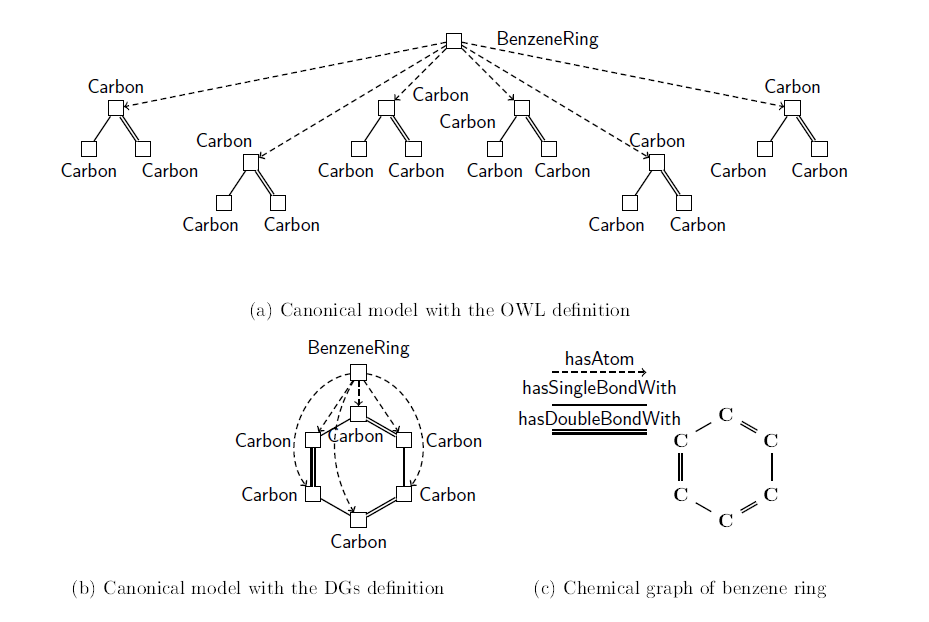
\includegraphics[width=\textwidth]{images/chemgraphimg.png}
\end{figure}



%%%%%%%%%%%%%%%%%%%%%%%%%%%%%%%%%%%
%%                               %%
%% Tables                        %%
%%                               %%
%%%%%%%%%%%%%%%%%%%%%%%%%%%%%%%%%%%

%% Use of \listoftables is discouraged.

\section*{Tables}


\subsection*{Table 1 -- Features used to define structure-based classes}
\label{tab:classes}
    Structure-based classes in chemistry are defined using the following features either singly or in composition with other features. \par \mbox{}
    \par
    \mbox{
      \begin{tabular}{|c|p{3cm}|p{5cm}|p{4cm}|}
        \hline %\multicolumn{3}{|c|}{Structure-based features for class definitions}\\ \hline
        \textbf{Abbreviation} & \textbf{Feature} & \textbf{Description}  & \textbf{Examples} \\ \hline
        IP.1 & Skeleton & The main carbon backbone of the molecule & porphyrins, pyridines  \\ \hline
        IP.2 & Attached group & A functional group attached in some position on the skeleton & metalloporphyrins   \\ \hline
        IP.3 & Arbitrary part & A group present in any position within the molecule & carboxylic acid   \\ \hline
        IP.4 & Count of parts & The specific number, or a constraint on the number, of parts of a specified type & tricarboxylic acid  \\ \hline
        IP.5 & Relative arrangement of parts & Relative arrangement of parts of a specified type & allothreonine, threonine  \\ \hline
        CP.1 & Basic chemical properties such as charge &  Presence of a specific number of charges, or unpaired electrons & anion, cation, dication \\ \hline
        AP.1 & Which atoms are present & Presence or absence of atoms of specified types arranged according to the periodic table & lanthanine molecular entities \\ \hline
        TF.1 & Topological features -- presence of cycles & Whether a molecule contains cycles of specified types & heterocyclic molecule \\ \hline
        TF.2 & Topological features -- count of cycles  & Presence of the specified number of distinct (smallest) cycles & bicyclic, tricyclic molecule \\ \hline
        TF.3 & Topological features -- interrelation between cycles (fusing, arrangements)  & Relative arrangements and fusing between cycles  & ortho-fused and peri-fused molecule \\ \hline
        TF.4 & Topological features & Overall aspects of connectivity, such as ring arrangements & Polycyclic cage, fullerene, nanotube \\ \hline
        MC.1 & Mechanical connectivity & Mechanical connectivity / interlocking & rotaxanes, catenanes \\ \hline
        MC.2 & Mechanical shape of molecule & Features of overall shape of molecule & molecular M\"{o}bius strips, molecular knots  \\ \hline
        SF.1 & Structural formula -- atomic & A schema for structural formulae in terms of the relative number of different types of atom & Hydrocarbons, alkanes \\ \hline
        SF.2 & Structural formula -- repeating substructural units (polymers) & Structural formulae in terms of relative numbers of substructural units & polyethylene, poly... \\ \hline
      \end{tabular}
      } 
%%%
%%% END TABLE


\subsection*{DL-safe rules example}
\begin{table}[h!]
\centering
\caption{DL-safe rules example}\label{tab:DL-safe-example}
\rowcolors{1}{tableShade}{white}
\begin{tabular}{|l|l|}
    \hline
    TBox axiom    & $\mathsf{\exists hasAtom.RingAtom \sqsubseteq CyclicMolecule}$ \\
    ABox axioms & $\mathsf{Benzene(m),singleBond(a_1,a_2),doubleBond(a_2,a_3),singleBond(a_3,a_4),doubleBond(a_4,a_5),}$ \\ 
     & $\mathsf{singleBond(a_5,a_6),doubleBond(a_6,a_1),Carbon(a_i),hasAtom(m,a_i)}$  for each $ 1 \leq \mathsf{i} \leq 6$ \\
     DL-safe rule &  $\mathsf{ \bigwedge_{1 \leq i \leq 6}   Carbon(x_i)   \wedge singleBond(x_1,x_2) \wedge doubleBond(x_2,x_3) \wedge singleBond(x_3,x_4)} \wedge{}$ \\
     & $\mathsf{doubleBond(x_4,x_5) \wedge singleBond(x_5,x_6) \wedge doubleBond(x_6,x_1) \rightarrow RingAtom(x_1)}$ \\
      
     \hline 
\end{tabular}
\end{table}
%


%%%%%%%%%%%%%%%%%%%%%%%%%%%%%%%%%%%
%%                               %%
%% Additional Files              %%
%%                               %%
%%%%%%%%%%%%%%%%%%%%%%%%%%%%%%%%%%%
\begin{comment}
\section*{Additional Files}
  \subsection*{Additional file 1 --- Sample additional file title}
    Additional file descriptions text (including details of how to
    view the file, if it is in a non-standard format or the file extension).  This might
    refer to a multi-page table or a figure.

  \subsection*{Additional file 2 --- Sample additional file title}
    Additional file descriptions text.
\end{comment}

\end{bmcformat}
\end{document}







